\pagebreak

\section{Pulse Code Modulation (PCM)}
\label{sec:Pulse Code Modulation (PCM)}

\subsection{Theory}

Pulse Code Modulation (PCM) is a technique used to digitize analog signals.
The process involves three main steps: sampling, quantization, and encoding.


\begin{enumerate}
      \item In the first step, the analog signal is sampled at regular intervals\footnote[1]{The Nyquist-Shannon sampling theorem states that a signal can be perfectly reconstructed from its samples if the sampling rate is at least twice the maximum frequency of the signal.}.
            The resulting sequence of samples represents the signal in a discrete-time domain.

      \item In the second step, the samples are quantized into a finite number of levels.
            This reduces the number of possible amplitude values that each sample can take on, resulting in a loss of information compared to the original analog signal.
            However, quantization allows for the signal to be represented using a fixed number of bits, which is necessary for digital storage and transmission.

      \item In the third step, the quantized samples are encoded into binary code words.
            Each code word represents a quantization level and is assigned a unique binary code based on the number of bits used to represent it.
            This is typically done using a lookup table that maps each quantization level to a binary code.
\end{enumerate}

To demodulate the signal, the process is reversed.

\subsection{Matlab Code}

\inputminted[fontsize=\footnotesize,autogobble]{matlab}{code/pcm.m}

\pagebreak
\subsection{Output}

\begin{figure}[!htb]
      \centering
      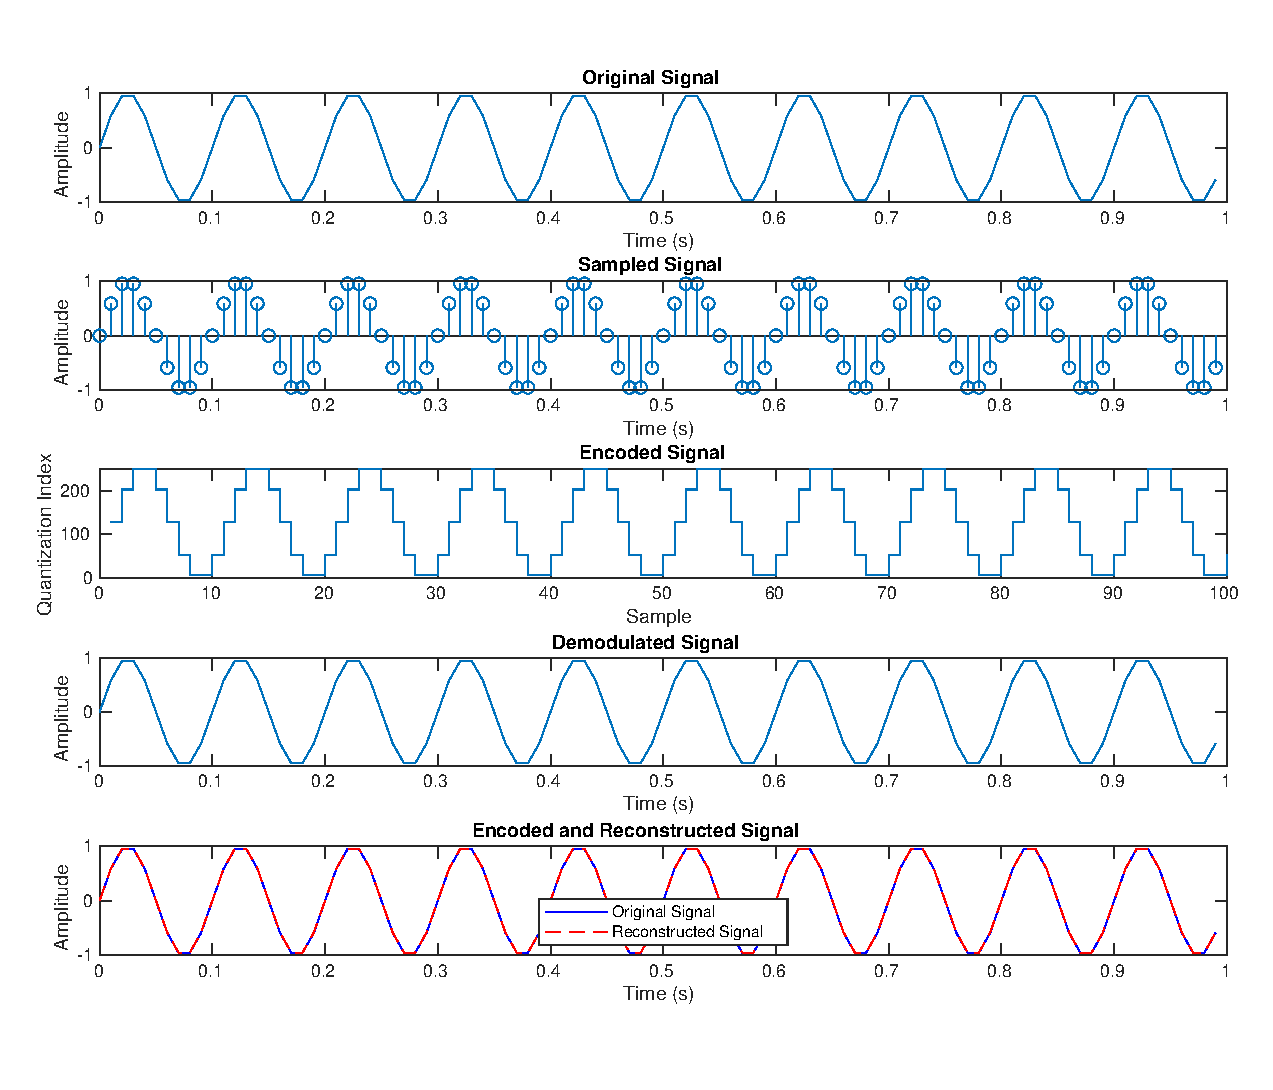
\includegraphics[width=\textwidth]{res/figures/pcm_no_quantization.pdf}
      \label{output:pcm}
      \caption{PCM}
\end{figure}
